\section{Benchmarks}
\label{sec:benchmarks}


%\begin{figure}[ht]
%	\centering
	\framebox{
		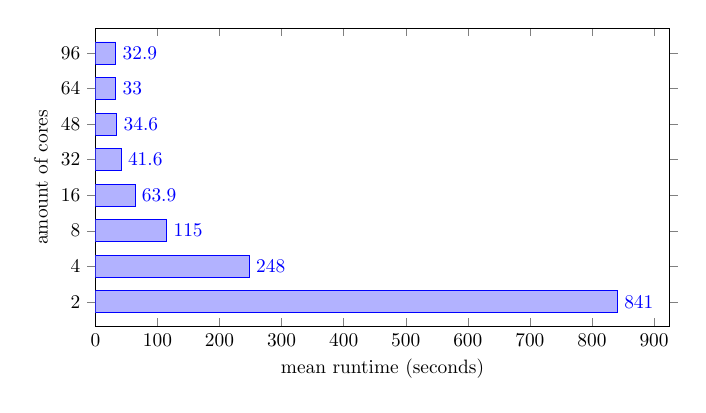
\begin{tikzpicture}[thick, scale=0.7]
		\begin{axis}[
			xbar, xmin=0,
			bar width=0.4cm,
			width=12cm, height=7cm, enlarge y limits=0.1,
			ylabel={amount of cores},
			xlabel={mean runtime (seconds)},
			symbolic y coords={2, 4, 8, 16, 32, 48, 64, 96},
			ytick=data,
			nodes near coords, nodes near coords align={horizontal},
			]
			\addplot coordinates {(841,2) (248,4) (115,8) (63.9,16) (41.6,32) (34.6,48) (33.0,64) (32.9,96)};
		\end{axis}
		\end{tikzpicture}
	}
%	\caption[Parallel Matrix Multiplication using Eden (two 1024x1024 matrices)]
%\end{figure}

\framebox{
	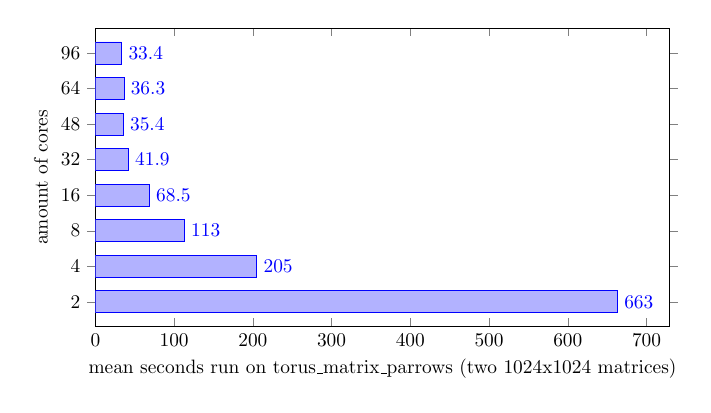
\begin{tikzpicture}[thick, scale=0.7]
	\begin{axis}[
	xbar, xmin=0,
	bar width=0.4cm,
	width=12cm, height=7cm, enlarge y limits=0.1,
	ylabel={amount of cores},
	xlabel={mean seconds run on torus\_matrix\_parrows (two 1024x1024 matrices)},
	symbolic y coords={2, 4, 8, 16, 32, 48, 64, 96},
	ytick=data,
	nodes near coords, nodes near coords align={horizontal},
	]
	\addplot coordinates {(663,2) (205,4) (113,8) (68.5,16) (41.9,32) (35.4,48) (36.3,64) (33.4,96)};
	\end{axis}
	\end{tikzpicture}
}


%%% Local Variables:
%%% mode: latex
%%% TeX-master: "main"
%%% End:
